\section{Introduction}



More and more applications are being deployed to the cloud, including real-time applications. Since cloud computing introduces non-deterministic latency\cite{rtcloud}, resources are usually over-provisioned for real-time applications to ensure performance requirements are met. On top of that, many real-time applications have dynamically varying workloads which result in greater resource under-utilization when the application is running in a lower workload mode. We can solve this problem by monitoring the status of the application and dynamically adjusting its resources. Since cloud computing relies heavily on virtualization, we are developing the Pacer framework in Xen. Pacer monitors real-time applications running in VMs and provides developers a platform on which they can implement their own choice of resource management scheme. The high level view of the Pacer framework is shown in figure \ref{anchors}, where the Pacer resource manager collects performance feedback and then dynamically adjust resource allocations for the VMs.
\begin{figure}[h!]
\centering
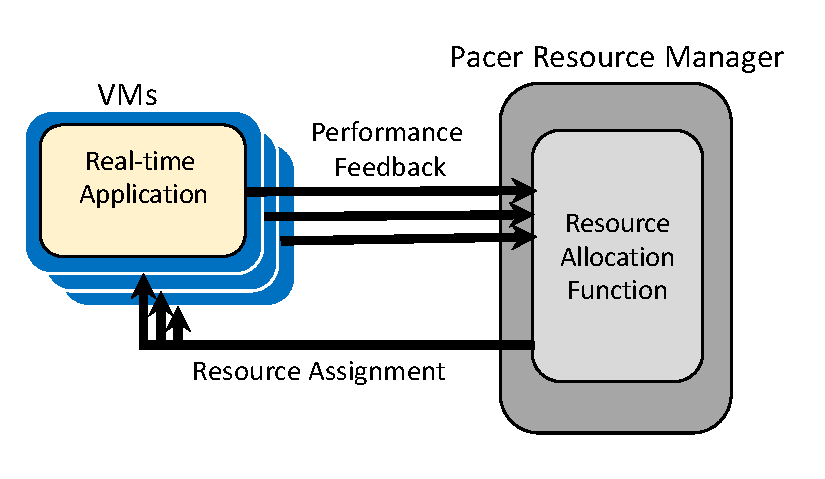
\includegraphics[width=1\linewidth]{images/anchors}
\caption{High Level Pacer Framework}
\label{anchors}
\end{figure}

A motivating example is a server hosting multiple VMs that run security surveillance applications monitoring different parts of a building. The application runs in a light workload mode when no intruder is detected, and switches to a heavier workload mode when an intruder is detected. While the application runs in the light workload mode, CPU resources can be saved for non real-time tasks such as routine server backups. When one or more cameras detect an intruder and switch to the heavier workload mode, Pacer becomes aware of the increased demand from the application and reassigns resource to the VMs such that all applications can meet their real-time performance requirements.

This paper makes the following contribution:
\begin{enumerate}
\item We develop Pacer, a framework that provides developers a platform to implement CPU resource allocation for VMs that run soft real-time applications.
\item We modify Additive-Increase-Multiplicative-Decrease\cite{aimd} and Self-Tuning PID Controller\cite{apid} and turn them into CPU resource allocation algorithms that utilizes feedback from real-time applications.
\item We present stride sharing, a CPU resource sharing algorithm based on stride scheduling\cite{stride} to improve real-time performance under an overloading system.
\end{enumerate}

The remainder of the paper is organized as follows: Section \ref{sr} presents related work. Section \ref{sb} presents background for the Pacer framework. Section \ref{sf} presents the details of the Pacer framework and its usage. Section \ref{sc} presents resource allocation and sharing algorithms. Section \ref{se} presents the experimental results and analysis. Finally, section \ref{send} presents our conclusions and future work.


